\documentclass{extbook}[14pt]
\usepackage{multicol, enumerate, enumitem, hyperref, color, soul, setspace, parskip, fancyhdr, amssymb, amsthm, amsmath, bbm, latexsym, units, mathtools}
\everymath{\displaystyle}
\usepackage[headsep=0.5cm,headheight=0cm, left=1 in,right= 1 in,top= 1 in,bottom= 1 in]{geometry}
\usepackage{dashrule}  % Package to use the command below to create lines between items
\newcommand{\litem}[1]{\item #1

\rule{\textwidth}{0.4pt}}
\pagestyle{fancy}
\lhead{}
\chead{Answer Key for Makeup Progress Quiz 1 Version B}
\rhead{}
\lfoot{6018-3080}
\cfoot{}
\rfoot{Spring 2021}
\begin{document}
\textbf{This key should allow you to understand why you choose the option you did (beyond just getting a question right or wrong). \href{https://xronos.clas.ufl.edu/mac1105spring2020/courseDescriptionAndMisc/Exams/LearningFromResults}{More instructions on how to use this key can be found here}.}

\textbf{If you have a suggestion to make the keys better, \href{https://forms.gle/CZkbZmPbC9XALEE88}{please fill out the short survey here}.}

\textit{Note: This key is auto-generated and may contain issues and/or errors. The keys are reviewed after each exam to ensure grading is done accurately. If there are issues (like duplicate options), they are noted in the offline gradebook. The keys are a work-in-progress to give students as many resources to improve as possible.}

\rule{\textwidth}{0.4pt}

\begin{enumerate}\litem{
Construct the lowest-degree polynomial given the zeros below. Then, choose the intervals that contain the coefficients of the polynomial in the form $ax^3+bx^2+cx+d$.
\[ \frac{-3}{2}, \frac{-6}{5}, \text{ and } \frac{7}{4} \]The solution is \( 40x^{3} +38 x^{2} -117 x -126 \), which is option A.\begin{enumerate}[label=\Alph*.]
\item \( a \in [40, 41], b \in [37, 46], c \in [-118, -115], \text{ and } d \in [-127, -124] \)

* $40x^{3} +38 x^{2} -117 x -126$, which is the correct option.
\item \( a \in [40, 41], b \in [-178, -176], c \in [250, 263], \text{ and } d \in [-127, -124] \)

$40x^{3} -178 x^{2} +261 x -126$, which corresponds to multiplying out $(2x -3)(5x -6)(4x -7)$.
\item \( a \in [40, 41], b \in [37, 46], c \in [-118, -115], \text{ and } d \in [126, 127] \)

$40x^{3} +38 x^{2} -117 x + 126$, which corresponds to multiplying everything correctly except the constant term.
\item \( a \in [40, 41], b \in [-47, -32], c \in [-118, -115], \text{ and } d \in [126, 127] \)

$40x^{3} -38 x^{2} -117 x + 126$, which corresponds to multiplying out $(2x -3)(5x -6)(4x + 7)$.
\item \( a \in [40, 41], b \in [-82, -80], c \in [-56, -48], \text{ and } d \in [126, 127] \)

$40x^{3} -82 x^{2} -51 x + 126$, which corresponds to multiplying out $(2x -3)(5x + 6)(4x -7)$.
\end{enumerate}

\textbf{General Comment:} To construct the lowest-degree polynomial, you want to multiply out $(2x + 3)(5x + 6)(4x -7)$
}
\litem{
Describe the end behavior of the polynomial below.
\[ f(x) = 6(x - 5)^{4}(x + 5)^{7}(x + 9)^{3}(x - 9)^{5} \]The solution is the graph below, which is option D.
\begin{center}
    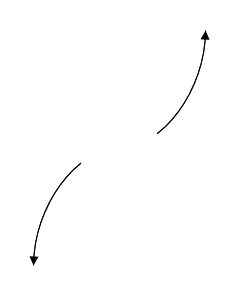
\includegraphics[width=0.3\textwidth]{../Figures/polyEndBehaviorDB.png}
\end{center}\begin{enumerate}[label=\Alph*.]
\begin{multicols}{2}
\item 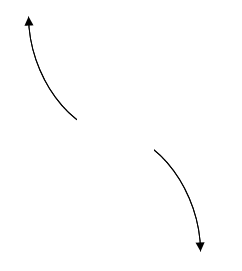
\includegraphics[width = 0.3\textwidth]{../Figures/polyEndBehaviorAB.png}
\item 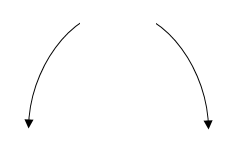
\includegraphics[width = 0.3\textwidth]{../Figures/polyEndBehaviorBB.png}
\item 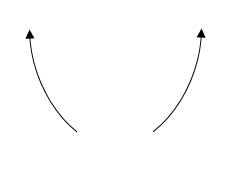
\includegraphics[width = 0.3\textwidth]{../Figures/polyEndBehaviorCB.png}
\item 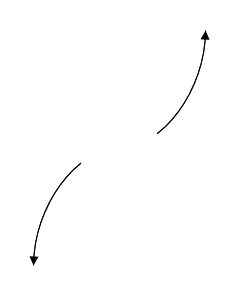
\includegraphics[width = 0.3\textwidth]{../Figures/polyEndBehaviorDB.png}
\end{multicols}\item None of the above.\end{enumerate}
\textbf{General Comment:} Remember that end behavior is determined by the leading coefficient AND whether the \textbf{sum} of the multiplicities is positive or negative.
}
\litem{
Construct the lowest-degree polynomial given the zeros below. Then, choose the intervals that contain the coefficients of the polynomial in the form $x^3+bx^2+cx+d$.
\[ -2 + 2 i \text{ and } 3 \]The solution is \( x^{3} + x^{2} -4 x -24 \), which is option A.\begin{enumerate}[label=\Alph*.]
\item \( b \in [0, 1.7], c \in [-4.1, -3.6], \text{ and } d \in [-27, -20] \)

* $x^{3} + x^{2} -4 x -24$, which is the correct option.
\item \( b \in [-3.8, 0.8], c \in [-4.1, -3.6], \text{ and } d \in [21, 27] \)

$x^{3} -1 x^{2} -4 x + 24$, which corresponds to multiplying out $(x-(-2 + 2 i))(x-(-2 - 2 i))(x + 3)$.
\item \( b \in [0, 1.7], c \in [-5.5, -4.1], \text{ and } d \in [6, 7] \)

$x^{3} + x^{2} -5 x + 6$, which corresponds to multiplying out $(x -2)(x -3)$.
\item \( b \in [0, 1.7], c \in [-3.9, 3.7], \text{ and } d \in [-9, -3] \)

$x^{3} + x^{2} -x -6$, which corresponds to multiplying out $(x + 2)(x -3)$.
\item \( \text{None of the above.} \)

This corresponds to making an unanticipated error or not understanding how to use nonreal complex numbers to create the lowest-degree polynomial. If you chose this and are not sure what you did wrong, please contact the coordinator for help.
\end{enumerate}

\textbf{General Comment:} Remember that the conjugate of $a+bi$ is $a-bi$. Since these zeros always come in pairs, we need to multiply out $(x-(-2 + 2 i))(x-(-2 - 2 i))(x-(3))$.
}
\litem{
Construct the lowest-degree polynomial given the zeros below. Then, choose the intervals that contain the coefficients of the polynomial in the form $ax^3+bx^2+cx+d$.
\[ \frac{7}{4}, \frac{1}{4}, \text{ and } \frac{2}{3} \]The solution is \( 48x^{3} -128 x^{2} +85 x -14 \), which is option D.\begin{enumerate}[label=\Alph*.]
\item \( a \in [44, 56], b \in [126, 137], c \in [81, 90], \text{ and } d \in [11, 17] \)

$48x^{3} +128 x^{2} +85 x + 14$, which corresponds to multiplying out $(4x + 7)(4x + 1)(3x + 2)$.
\item \( a \in [44, 56], b \in [-135, -118], c \in [81, 90], \text{ and } d \in [11, 17] \)

$48x^{3} -128 x^{2} +85 x + 14$, which corresponds to multiplying everything correctly except the constant term.
\item \( a \in [44, 56], b \in [63, 68], c \in [-46, -41], \text{ and } d \in [-14, -7] \)

$48x^{3} +64 x^{2} -43 x -14$, which corresponds to multiplying out $(4x + 7)(4x + 1)(3x -2)$.
\item \( a \in [44, 56], b \in [-135, -118], c \in [81, 90], \text{ and } d \in [-14, -7] \)

* $48x^{3} -128 x^{2} +85 x -14$, which is the correct option.
\item \( a \in [44, 56], b \in [39, 42], c \in [-69, -65], \text{ and } d \in [11, 17] \)

$48x^{3} +40 x^{2} -69 x + 14$, which corresponds to multiplying out $(4x + 7)(4x -1)(3x -2)$.
\end{enumerate}

\textbf{General Comment:} To construct the lowest-degree polynomial, you want to multiply out $(4x -7)(4x -1)(3x -2)$
}
\litem{
Construct the lowest-degree polynomial given the zeros below. Then, choose the intervals that contain the coefficients of the polynomial in the form $x^3+bx^2+cx+d$.
\[ 2 - 3 i \text{ and } -2 \]The solution is \( x^{3} -2 x^{2} +5 x + 26 \), which is option D.\begin{enumerate}[label=\Alph*.]
\item \( b \in [0.54, 1.9], c \in [-1, 4], \text{ and } d \in [-4, -2] \)

$x^{3} + x^{2} -4$, which corresponds to multiplying out $(x -2)(x + 2)$.
\item \( b \in [1.49, 3.68], c \in [5, 7], \text{ and } d \in [-31, -17] \)

$x^{3} +2 x^{2} +5 x -26$, which corresponds to multiplying out $(x-(2 - 3 i))(x-(2 + 3 i))(x -2)$.
\item \( b \in [0.54, 1.9], c \in [5, 7], \text{ and } d \in [4, 8] \)

$x^{3} + x^{2} +5 x + 6$, which corresponds to multiplying out $(x + 3)(x + 2)$.
\item \( b \in [-2.47, -1.16], c \in [5, 7], \text{ and } d \in [19, 30] \)

* $x^{3} -2 x^{2} +5 x + 26$, which is the correct option.
\item \( \text{None of the above.} \)

This corresponds to making an unanticipated error or not understanding how to use nonreal complex numbers to create the lowest-degree polynomial. If you chose this and are not sure what you did wrong, please contact the coordinator for help.
\end{enumerate}

\textbf{General Comment:} Remember that the conjugate of $a+bi$ is $a-bi$. Since these zeros always come in pairs, we need to multiply out $(x-(2 - 3 i))(x-(2 + 3 i))(x-(-2))$.
}
\litem{
Which of the following equations \textit{could} be of the graph presented below?

\begin{center}
    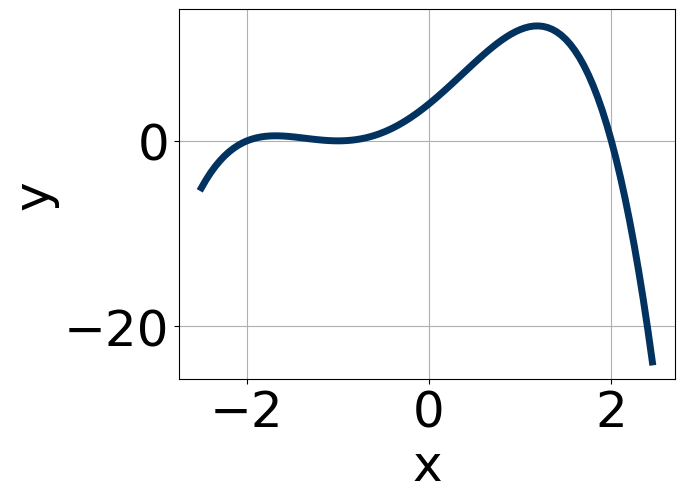
\includegraphics[width=0.5\textwidth]{../Figures/polyGraphToFunctionB.png}
\end{center}


The solution is \( -9(x + 1)^{6} (x + 2)^{11} (x - 2)^{5} \), which is option B.\begin{enumerate}[label=\Alph*.]
\item \( -11(x + 1)^{10} (x + 2)^{10} (x - 2)^{7} \)

The factor $(x + 2)$ should have an odd power.
\item \( -9(x + 1)^{6} (x + 2)^{11} (x - 2)^{5} \)

* This is the correct option.
\item \( 4(x + 1)^{8} (x + 2)^{5} (x - 2)^{9} \)

This corresponds to the leading coefficient being the opposite value than it should be.
\item \( -14(x + 1)^{5} (x + 2)^{6} (x - 2)^{5} \)

The factor $-1$ should have an even power and the factor $-2$ should have an odd power.
\item \( 10(x + 1)^{8} (x + 2)^{11} (x - 2)^{8} \)

The factor $(x - 2)$ should have an odd power and the leading coefficient should be the opposite sign.
\end{enumerate}

\textbf{General Comment:} General Comments: Draw the x-axis to determine which zeros are touching (and so have even multiplicity) or cross (and have odd multiplicity).
}
\litem{
Describe the zero behavior of the zero $x = 7$ of the polynomial below.
\[ f(x) = 5(x + 5)^{12}(x - 5)^{8}(x - 7)^{10}(x + 7)^{5} \]The solution is the graph below, which is option C.
\begin{center}
    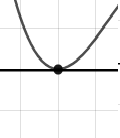
\includegraphics[width=0.3\textwidth]{../Figures/polyZeroBehaviorCopyCB.png}
\end{center}\begin{enumerate}[label=\Alph*.]
\begin{multicols}{2}
\item 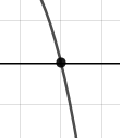
\includegraphics[width = 0.3\textwidth]{../Figures/polyZeroBehaviorCopyAB.png}
\item 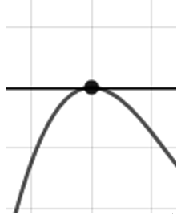
\includegraphics[width = 0.3\textwidth]{../Figures/polyZeroBehaviorCopyBB.png}
\item 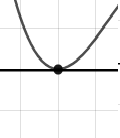
\includegraphics[width = 0.3\textwidth]{../Figures/polyZeroBehaviorCopyCB.png}
\item 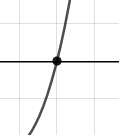
\includegraphics[width = 0.3\textwidth]{../Figures/polyZeroBehaviorCopyDB.png}
\end{multicols}\item None of the above.\end{enumerate}
\textbf{General Comment:} You will need to sketch the entire graph, then zoom in on the zero the question asks about.
}
\litem{
Describe the end behavior of the polynomial below.
\[ f(x) = -8(x + 7)^{2}(x - 7)^{3}(x + 5)^{2}(x - 5)^{3} \]The solution is the graph below, which is option B.
\begin{center}
    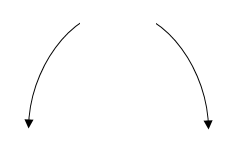
\includegraphics[width=0.3\textwidth]{../Figures/polyEndBehaviorCopyBB.png}
\end{center}\begin{enumerate}[label=\Alph*.]
\begin{multicols}{2}
\item 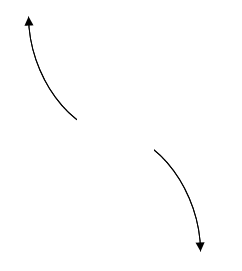
\includegraphics[width = 0.3\textwidth]{../Figures/polyEndBehaviorCopyAB.png}
\item 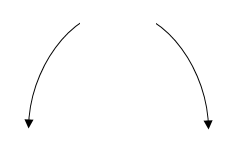
\includegraphics[width = 0.3\textwidth]{../Figures/polyEndBehaviorCopyBB.png}
\item 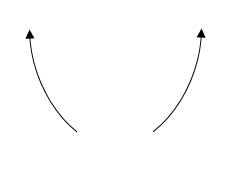
\includegraphics[width = 0.3\textwidth]{../Figures/polyEndBehaviorCopyCB.png}
\item 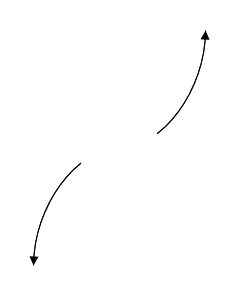
\includegraphics[width = 0.3\textwidth]{../Figures/polyEndBehaviorCopyDB.png}
\end{multicols}\item None of the above.\end{enumerate}
\textbf{General Comment:} Remember that end behavior is determined by the leading coefficient AND whether the \textbf{sum} of the multiplicities is positive or negative.
}
\litem{
Which of the following equations \textit{could} be of the graph presented below?

\begin{center}
    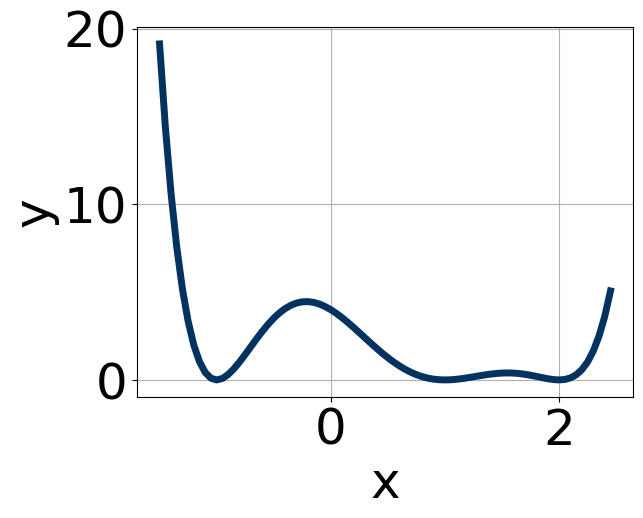
\includegraphics[width=0.5\textwidth]{../Figures/polyGraphToFunctionCopyB.png}
\end{center}


The solution is \( 2(x - 2)^{4} (x - 1)^{4} (x + 1)^{6} \), which is option D.\begin{enumerate}[label=\Alph*.]
\item \( 14(x - 2)^{8} (x - 1)^{7} (x + 1)^{5} \)

The factors $(x - 1)$ and $(x + 1)$ should both have even powers.
\item \( 12(x - 2)^{4} (x - 1)^{10} (x + 1)^{9} \)

The factor $(x + 1)$ should have an even power.
\item \( -3(x - 2)^{6} (x - 1)^{10} (x + 1)^{8} \)

This corresponds to the leading coefficient being the opposite value than it should be.
\item \( 2(x - 2)^{4} (x - 1)^{4} (x + 1)^{6} \)

* This is the correct option.
\item \( -6(x - 2)^{10} (x - 1)^{4} (x + 1)^{9} \)

The factor $(x + 1)$ should have an even power and the leading coefficient should be the opposite sign.
\end{enumerate}

\textbf{General Comment:} General Comments: Draw the x-axis to determine which zeros are touching (and so have even multiplicity) or cross (and have odd multiplicity).
}
\litem{
Describe the zero behavior of the zero $x = 8$ of the polynomial below.
\[ f(x) = -5(x + 3)^{7}(x - 3)^{5}(x + 8)^{6}(x - 8)^{3} \]The solution is the graph below, which is option A.
\begin{center}
    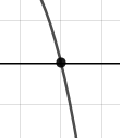
\includegraphics[width=0.3\textwidth]{../Figures/polyZeroBehaviorAB.png}
\end{center}\begin{enumerate}[label=\Alph*.]
\begin{multicols}{2}
\item 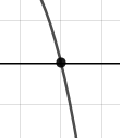
\includegraphics[width = 0.3\textwidth]{../Figures/polyZeroBehaviorAB.png}
\item 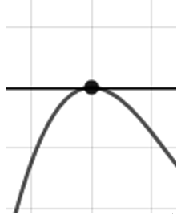
\includegraphics[width = 0.3\textwidth]{../Figures/polyZeroBehaviorBB.png}
\item 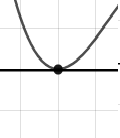
\includegraphics[width = 0.3\textwidth]{../Figures/polyZeroBehaviorCB.png}
\item 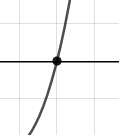
\includegraphics[width = 0.3\textwidth]{../Figures/polyZeroBehaviorDB.png}
\end{multicols}\item None of the above.\end{enumerate}
\textbf{General Comment:} You will need to sketch the entire graph, then zoom in on the zero the question asks about.
}
\end{enumerate}

\end{document}